\documentclass[english]{tktltiki}
\usepackage[pdftex]{graphicx}
\usepackage{subfigure}
\usepackage{url}
\usepackage{enumerate}
\begin{document}
%\doublespacing
%\singlespacing
\onehalfspacing

\title{Location Awareness - Week 2}
\author{P�ter Ivanics}
\date{\today}

\maketitle

\numberofpagesinformation{\numberofpages\ pages + \numberofappendixpages\ appendices}
\keywords{}

\mytableofcontents

\section{Coordinate Systems and Projections}

\begin{enumerate}[a)]
	\item 
	To determine ones position, it is essential to know the actual altitude of the object. The sea level is a good reference for the altitude, however due to the gravitational effects, the actual sea level might differ around the Earth. 
	
	The geoid is a hypothetical figure that approximates the mean sea level around the Earth as well as its shape. This yields in a mathematically indescribable shape and therefore cannot be used for determining ones position.
	
	The reference ellipsoid is the model of the geoid, which is utilized for mathematical calculations to determine ones position. This means that the shape is not totally accurate, it is only a fit to the geoid. If the mean sea level determined with this technique naturally includes some errors but afterall gives a good enough fit estimation on the position. This means, we can determine the position of an object with a tolerable error rate using an approximate surface of the Earth.
	
	\item 
	We talk about distortions when the 3-dimensional shape of the Earth is represented on a 2-dimensional surface. Distortion in this context is the unwanted alternation of the proportions on the 2-dimensional representation. This means, that some areas in the plane representation are not accurate, their real proportions differ due to deformation patterns. Depending on the selected projections, different distortions may occur. Three of these are, as follows: 
	
	\begin{itemize}
		\item scale distortion means that the proportion of the distance between two points are not accurate, for example in real life is 5 kilometer but on the map scale it appears to be two times larger or smaller,
		\item distance distortion refers to the error in the distance between two points caused by the distortion, for instance appears to be 2.5 kilometers when in reality is 5 kilometers,
		\item angular distortion means the change in a shape after the map projection, for instance when a circle appears as an ellipse.
	\end{itemize}
	\item The Mercator and the Transverse Mercator projections are both Cylindrical map projection methods. The main difference between them is caused by the fact that the former creates the projection with the Earth's equator touching the cylinder, while the latter rotates the cylinder by 90� with respect to rotation axis of the planet. This yields in different types of distortions for bot projections: 
	\begin{itemize}
		\item the Mercator suffers large objects with respect to their scale (e.g. the poles appear larger than they actually are),
		\item the Transverse Mercator distorts shapes and areas at extreme longitudes (e.g. South America appears larger).
	\end{itemize}
	
	Both projections are conformal. The former is the most known and used technique to project the map of the Earth.
\end{enumerate}

\section{KML Visualization}
	For solving this task, two small programs were developed. For the a) and b) parts, the attached $KMLGenerator.playground$ was implemented in Swift language. This program loads the points of the given CSV file and converts them into a valid KML file. The attached $points\_as\_placemarks.kml$ file contains the points for the a) part. A visual representation of the points is displayed on Figure \ref{points-as-placemarks}. The attached $points\_as\_linestring.kml$ file contains the output of the program. A visual representation of the points is displayed on Figure \ref{points-as-line}.
	
	\begin{figure}
		\begin{center}
			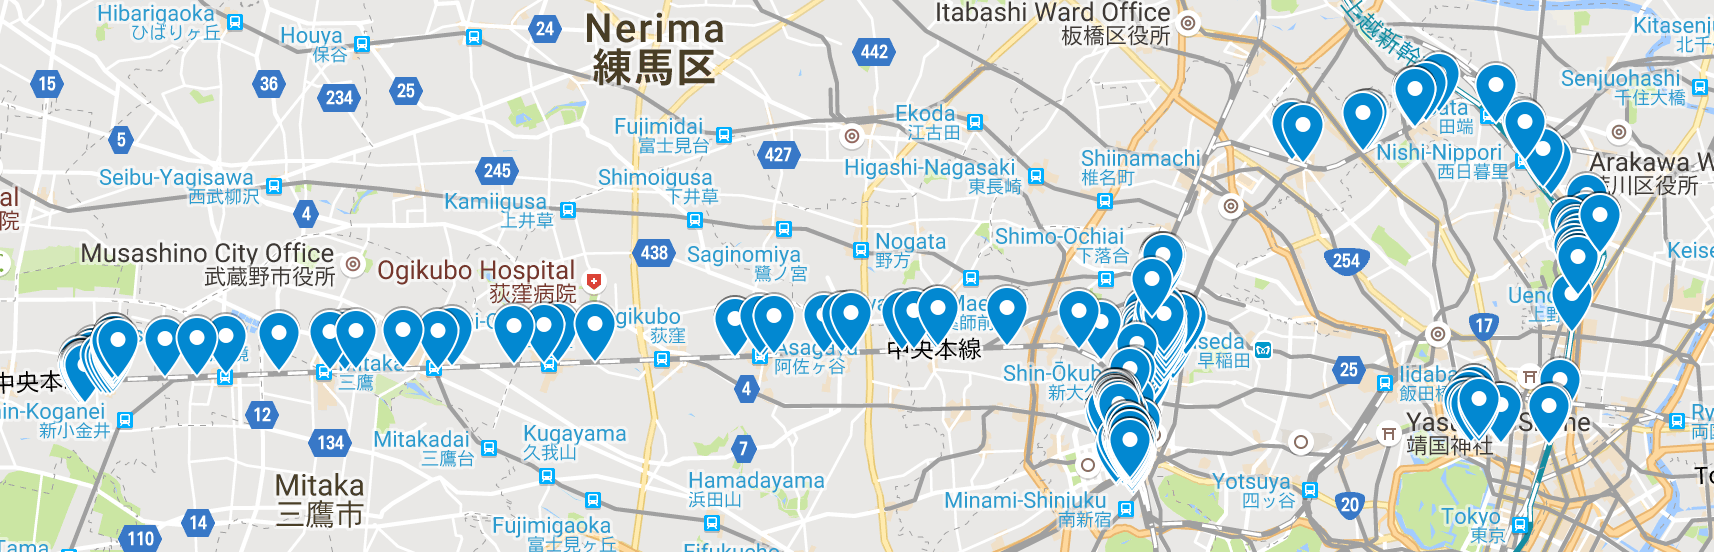
\includegraphics[width=0.9\textwidth]{images/points-as-placemarks.png}
			\caption{The given points represented on the Google Maps.}
			\label{points-as-placemarks} 
			
			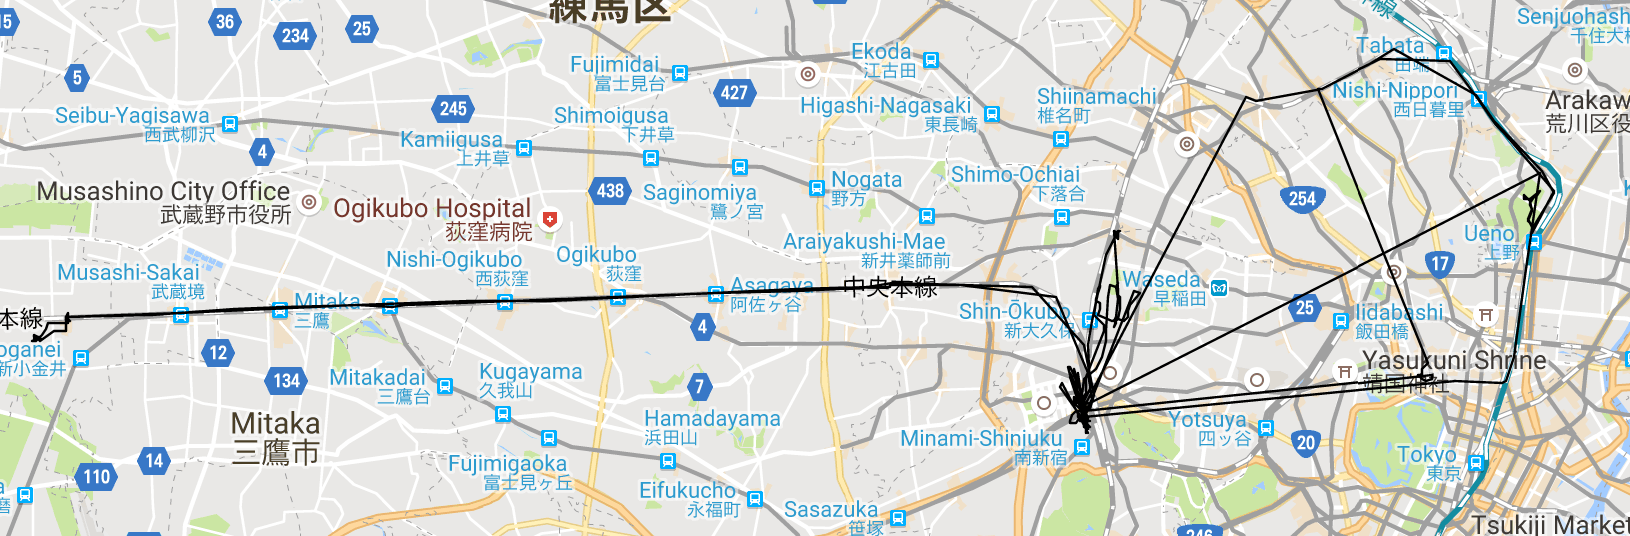
\includegraphics[width=0.9\textwidth]{images/points-as-line.png}
			\caption{The given points represented on the Google Maps connected with a line in their order of appearance.}
			\label{points-as-line}
		\end{center}
	\end{figure}
	
	For the c) part, the attached $add\_gaussian\_white\_noise.R$ was implemented in R language. A visual representation of the points is displayed on Figure \ref{points_with_white_noise}. On the left side the original points without noise are displayed, while on the right side the original points (with black dots) and the new points or noise is displayed (with red dots).

	\begin{figure}[h]
		\begin{center}
			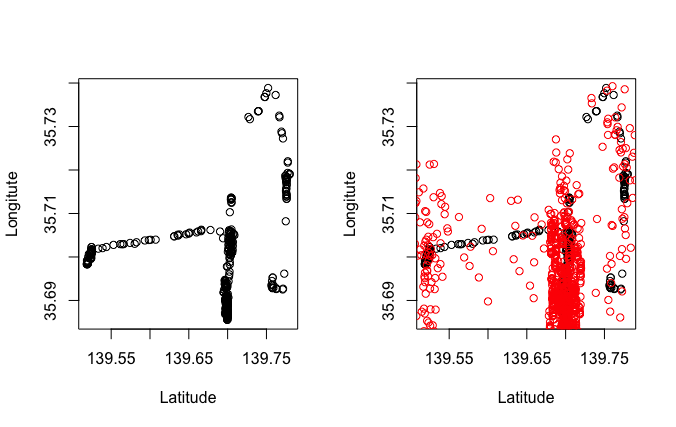
\includegraphics[width=0.9\textwidth]{images/points_with_white_noise.png}
			\caption{The given points represented in a standard plot (left) and the same points with randomly added zero-mean white noise (right, the noise displayed with red dots).}
			\label{points_with_white_noise}
		\end{center}
	\end{figure}

\pagebreak

\section{Fingerprint-based positioning}

\begin{enumerate}[a)]
	\item 
	\item 
\end{enumerate}

\section{Positioning implementation}

\nocite{*}
\bibliographystyle{tktl}
\bibliography{lahteet}

\lastpage

\appendices

\pagestyle{empty}

%\internalappendix{1}{Model ABC}
%
%The appendices here are just models of the table of contents and the presentation. Each appendix 
%usually starts on its own page, with the name and number of the appendix at the top. Each appendix is paginated separately.
%
%In addition to complementing the main document, each appendix is also its own, independent entity. 
%This means that an appendix cannot be just an image or a piece of programming, but the appendix must explain its contents and meaning.

\end{document}